\documentclass{article}

\usepackage{url}
\usepackage{tikz}
\usepackage{float}
\usepackage{amsmath}
\usepackage{enumitem}
\usepackage{graphicx}
\usepackage[outdir=./]{epstopdf}

\usetikzlibrary{matrix, shapes, snakes, arrows}
\tikzset{>=triangle 45}

\title{CS 612: Assignment 1\\Summer 2014}

\author{Dustin Ingram}

\date{\today}

\begin{document}

\maketitle

\section*{Written}


\begin{enumerate}

\item{} % a

Raising the minimum ideal temperature to 30,000 and the maximum to 31,000
results in a bug behavior which has very little movement, as the bugs are more
likely to be comfortable in their existing location. Lowering the minimum
temperature to 17,000 and the maximum to 18,000 results in a behavior with much
more individual movement, which in turn results in the heat gradient being
spread over the system more evenly.

\item{} % b

The ability to model our physical environment and related phenomena as cellular
automata would rely on the ability to reduce any physical phenomenon to a
series of predicable interactions between discrete particles. This leads to a
discussion of whether all elements of any physical phenomenon can truly be
considered discrete, but, assuming they are, it would be possible (in theory)
to model them after cellular automata.

\end{enumerate}

\newpage

\section*{Programming}

\emph{Note: all graphs and data are averaged over a 100-simulation run}

\begin{enumerate}

\item{} % 1

This graph shows the average distance between HeatBugs vs Time Step. As we see,
the average distance decreases over time, indicating that the bugs in this
particular model (the default) prefer to be slightly closer together than they
are originally set to be.

\begin{figure}[H]
\centering
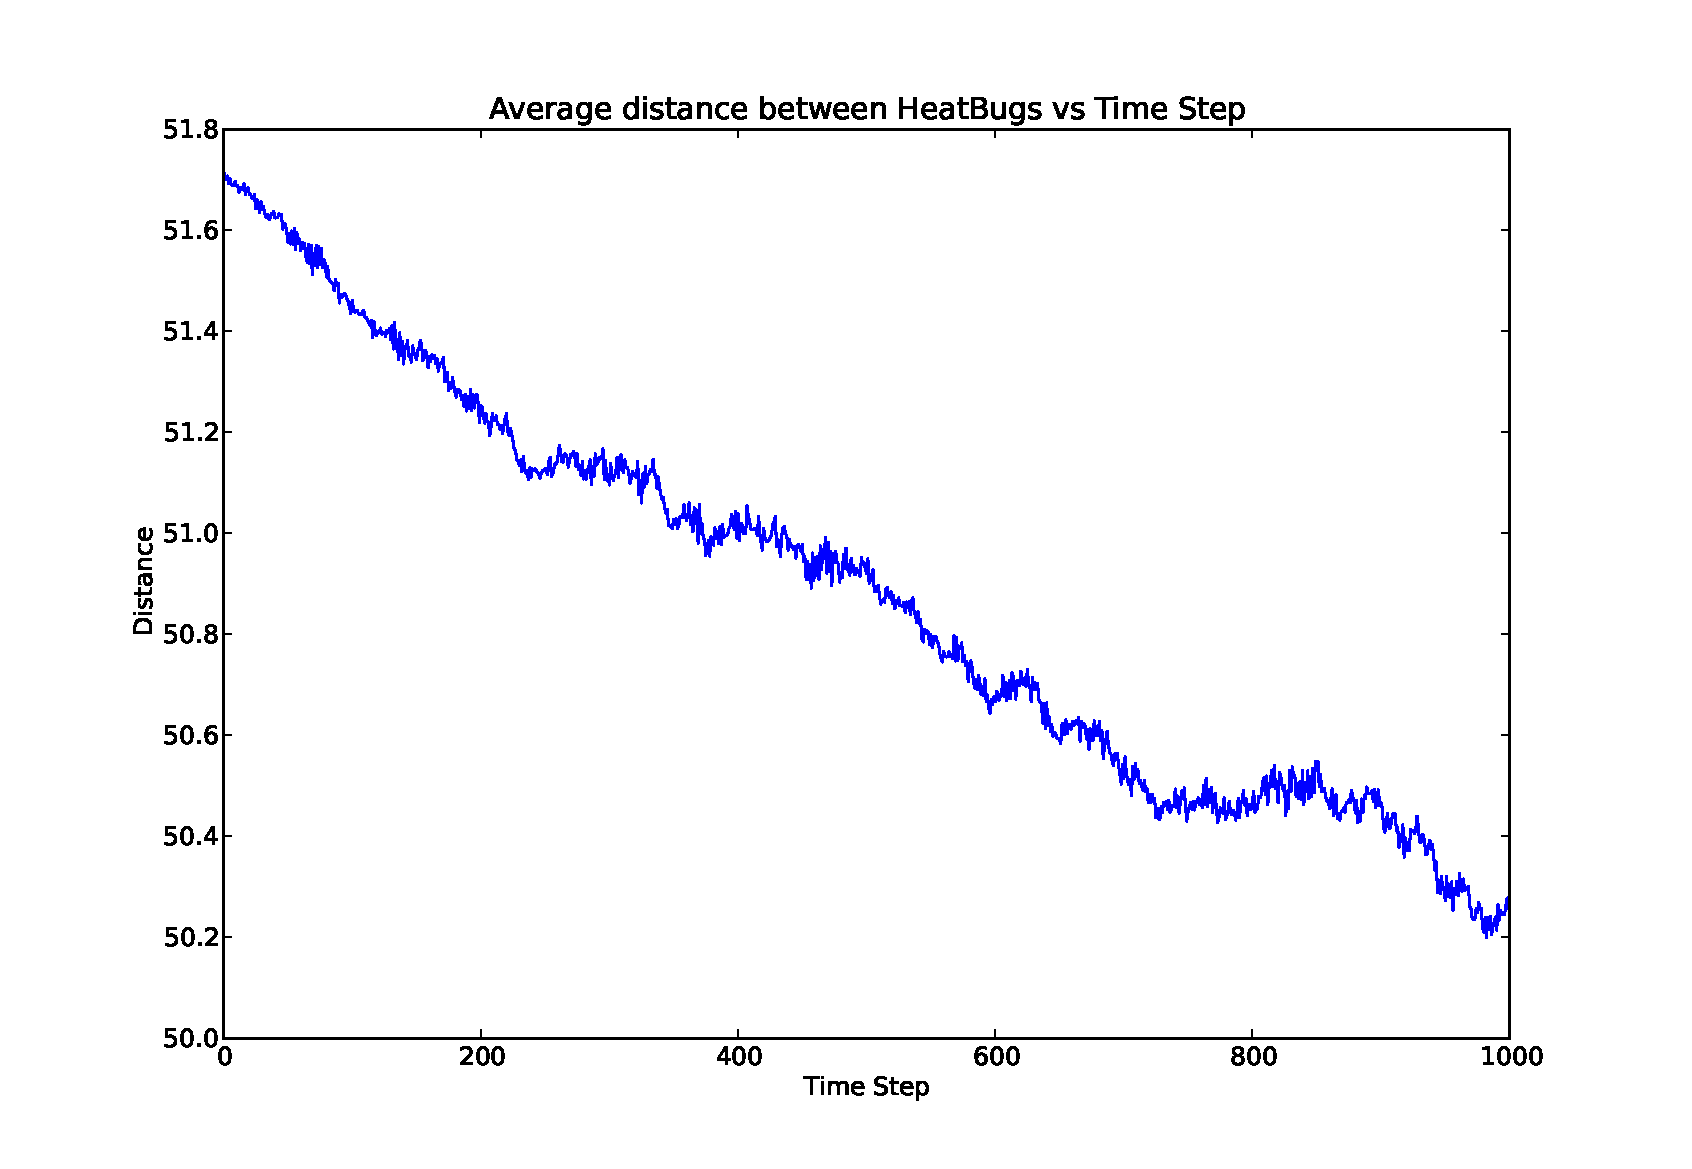
\includegraphics[width=\textwidth]{figs/figure_1}
\caption{Average distance between HeatBugs vs TimeStep}
\end{figure}

\newpage

\item{} % 2

This graph shows the average distance to each HeatBug's X closest neighbors at
timestep 1000 vs X. It reveals that, expectedly, the average distance between X
closest neighbors increases as X increases, due to the bugs tendency to
cluster.

\begin{figure}[H]
\centering
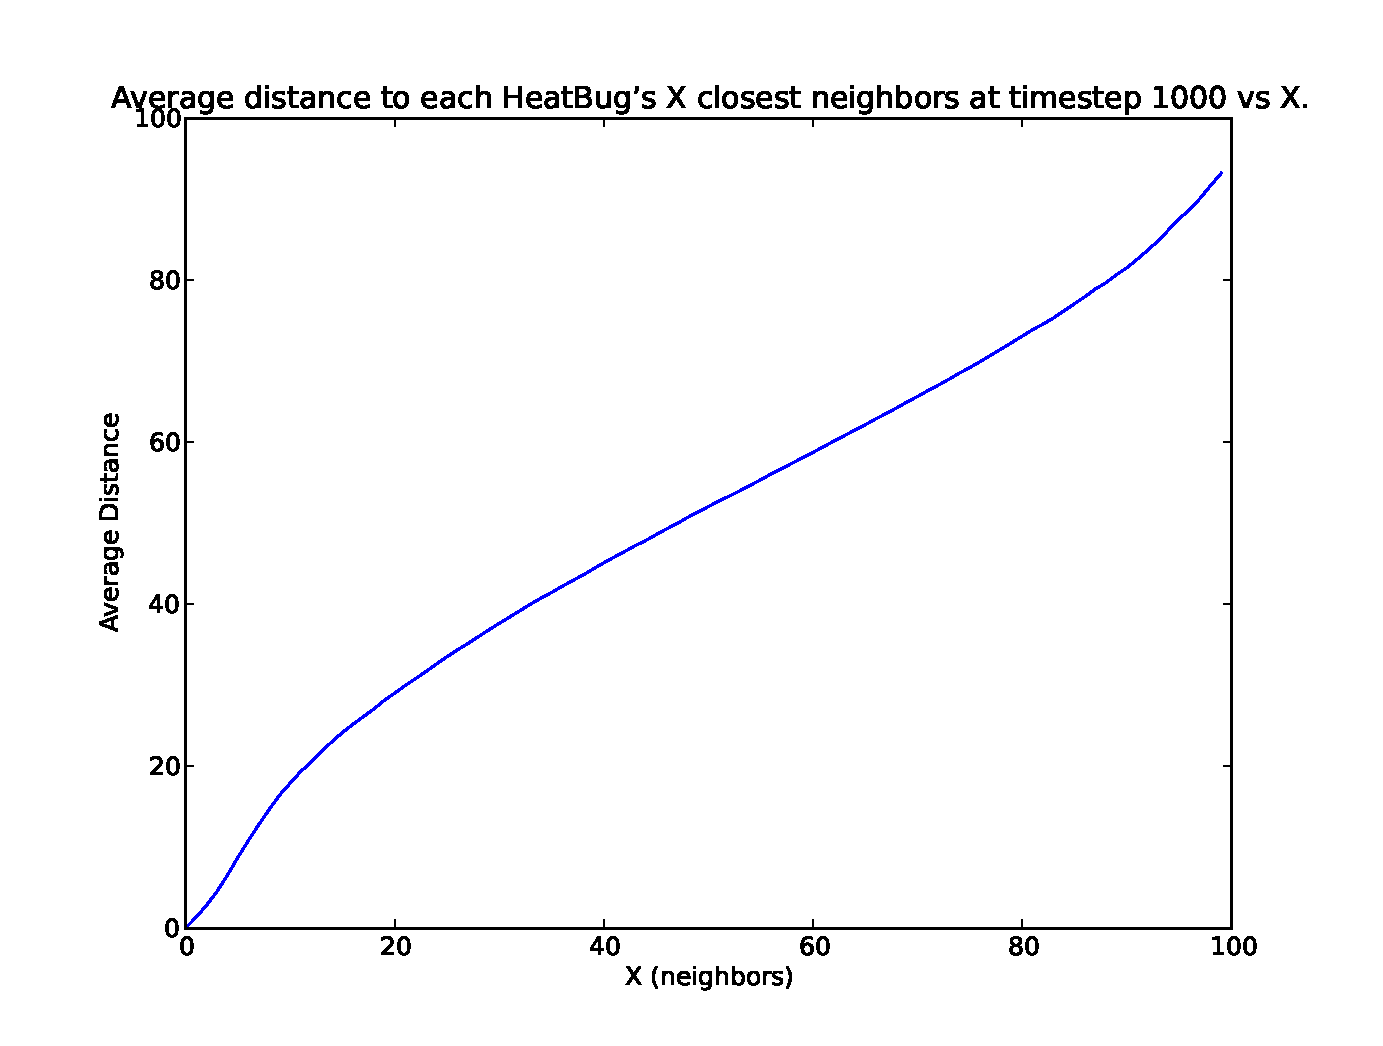
\includegraphics[width=\textwidth]{figs/figure_2}
\caption{Average distance to each HeatBug's X closest neighbors at timestep 1000 vs X.}
\end{figure}

\newpage

\item{} % 3

This graph shows the average distance to all other bugs vs ideal temperature.
While it shows that there is some variability in the distance based on the
ideal temperature, there is not a clear pattern here, due to the fact that the
bugs in the default scenario are close to uniformly scattered. Instead, it
might have been better to inspect the average distance for a set of X closest
neighbors, where this number is based on information collected in the previous
graph.

\begin{figure}[H]
\centering
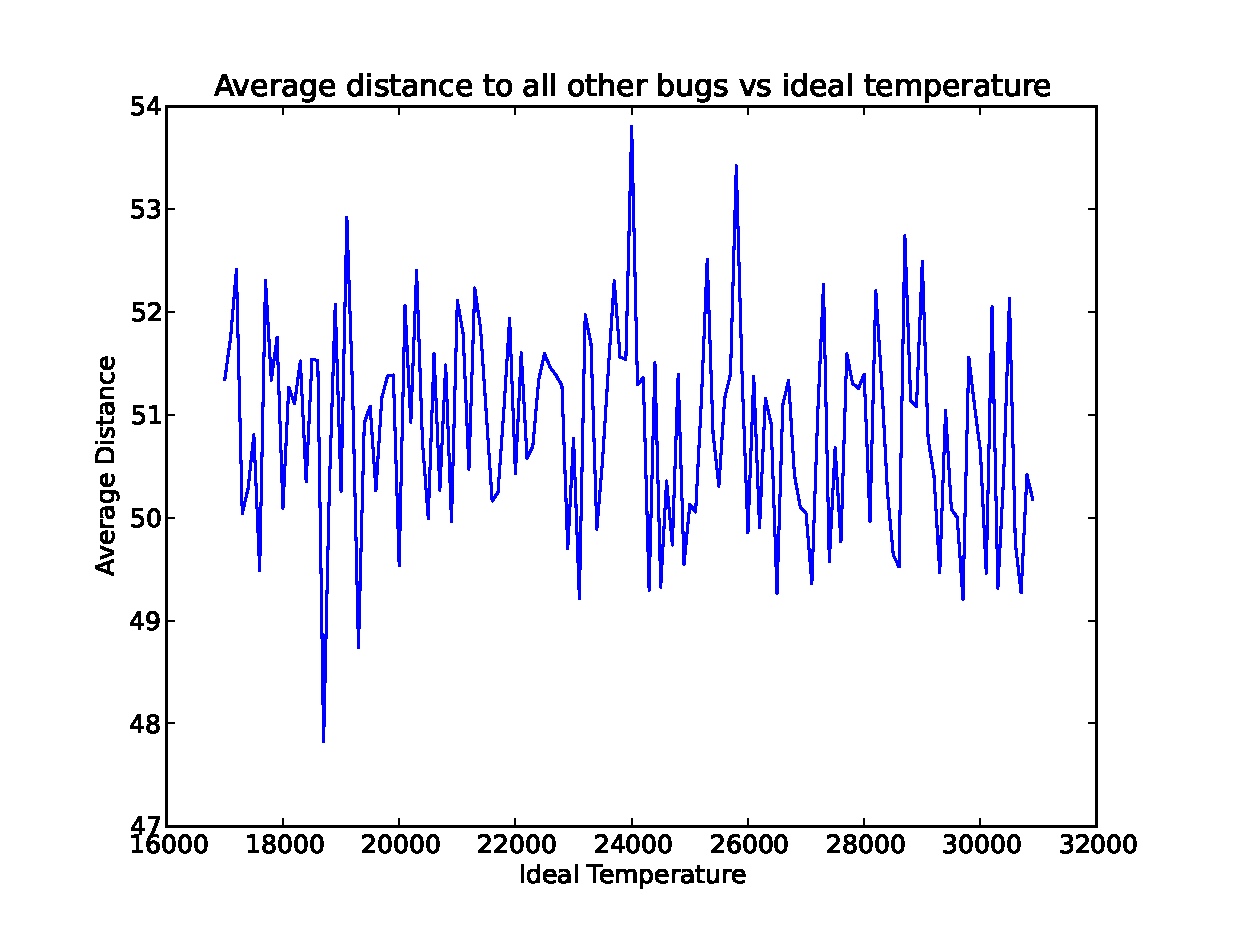
\includegraphics[width=\textwidth]{figs/figure_3}
\caption{Average distance to all other bugs vs ideal temperature}
\end{figure}

\newpage

\setcounter{enumi}{6}
\setcounter{figure}{6}

\item{} % 6

This graph attempts to show the relationship between the number of ``clusters''
in the system and the change over time. I attempted to use a agglomerative
clustering algorithm using the Euclidian distance between bugs, which allowed
for a non-predetermined number of clusters. I then used a threshold (~1\% of
the mean distance between all bugs) to determine the number of clusters. The
resulting graph could use a regression but the result is still clear--in this
example, regardless of how finely tuned the threshold is, the bugs become more
clustered over time.

\begin{figure}[H]
\centering
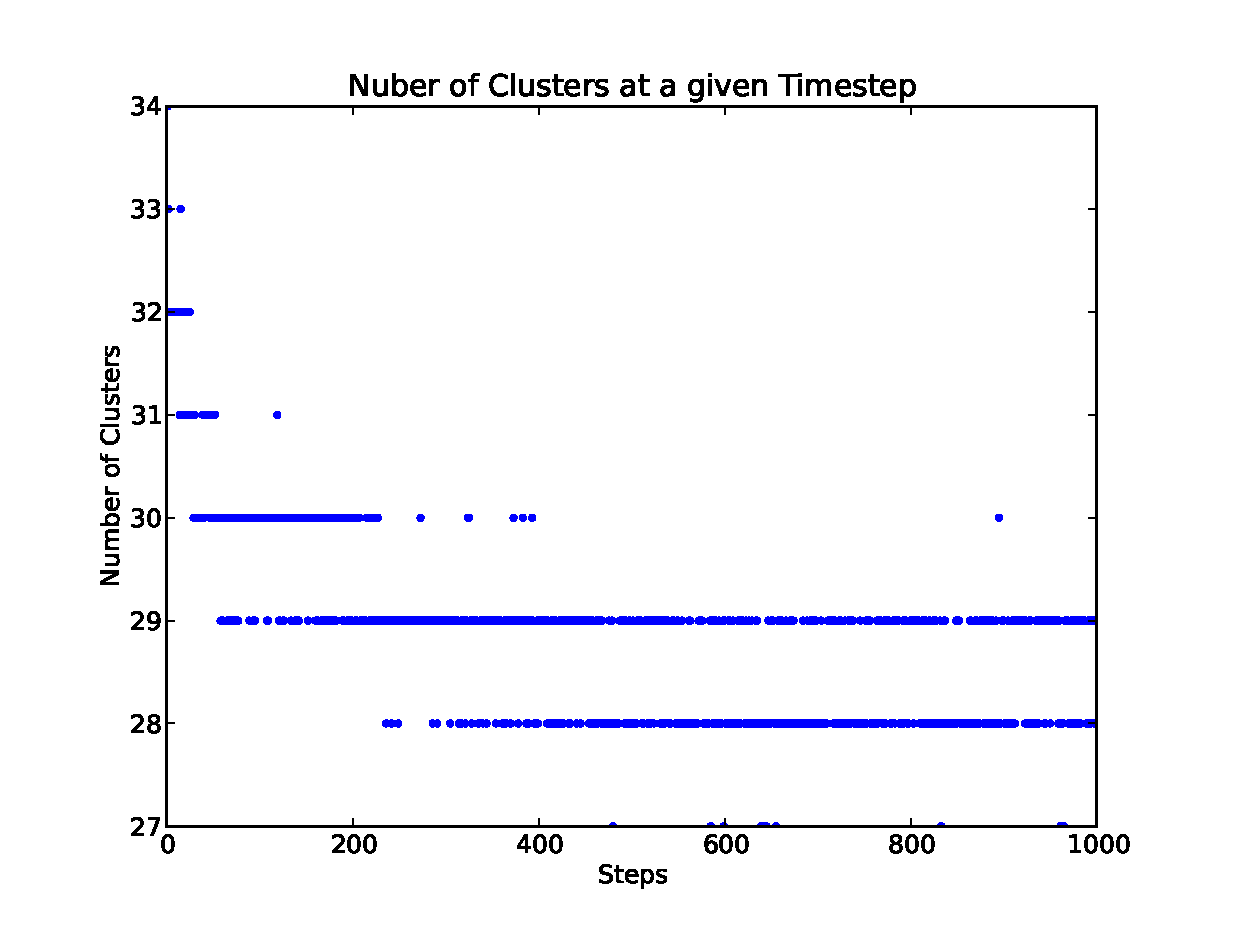
\includegraphics[width=\textwidth]{figs/figure_6}
\caption{Average number of clusters at every timestep}
\end{figure}


\item{} % 7

Not completed

\item{} % 8
I implemented this. The IceBug class is an exact copy of the HeatBug class,
with the exception that an IceBug removes heat instead of adding it to the
simulation. I also needed to create an abstract Bugs class that encapsulates
both Bug types. In addition, I modified the presentation of the bugs to color
them differently: HeatBugs remain the same (white) while IceBugs are,
obviously, blue. The number of bugs is split evenly for a total of 100 bugs.
The simulation can be run by running \texttt{java
sim.app.heatbugs.IceBugsWithUI}.

The result was interesting, the bugs essentially paired off into groups
consisting of one HeatBug for every IceBug, and stayed in very compact
clusters, and would combine clusters very quickly as well.


\end{enumerate}

\end{document}
